\chapter{Arka简要介绍}
Arka是一种人造语言.1991年始,她从零开始设计,处处都可以见到精巧的构思,在人文科学,哲学和语言学方面都有涉及.
现在她已经有一万六千余词,并且有自己的世界-Kaldia.

作为一门先验语,她的思路和世界语迥然不同,没有从英语,日语,汉语等现有语言做任何的借词.
她的所有词汇,都是,从草稿开始,进行词源的衍生和流变,一步一步发展起来的.
要知道,大多数创作者无法支撑这样一个庞大的先验语系,所以多采用后验方法构词,或是只建立一个很小的先验词汇表.
另外的一系是走工程语言的路线,像是John Wilkins的"真字".
\footnote{Real Character,由John Wilkins(1614-1672)建立的一门先验语,
其方向是成为一门世界辅助语,供学术和外交使用.
详见
\textattachfile{attachfiles/an essay towards a real character.7z}
{An Essay Towards a Real Character, and a Philosophical Language (London, 1668)}
这本书实在是太老又太大,译者无暇仔细阅读,但是将HTML格式的书打包成7z附于书中,供有心人参考.
}
能到Arka这样一万六千余词的规模,囊括世界观和文化细节\footnote{甚至有专门的章节讲述魔法的进化历程},实属不易.

Arka是一门在Kaldia讲述的艺术语,但也可以被地球人言说.
官网的建立者就是讲着日语,芬兰语,爱沙尼亚语,法语和德语等的总计30余人,
学习者更是遍布日,韩,中,英,美诸国.
至现在,学习者数量已有三倍的增长.


\section{开始}
读者可以看``诗姬和悠姬的一点Arka动画'',这是大概10分钟的动画.
\footnote{视频在YouTube上,官网的播放器已经不顶用了}
没有时间或者不方便的话,可以看这一章介绍的图.
\begin{figure}[H]
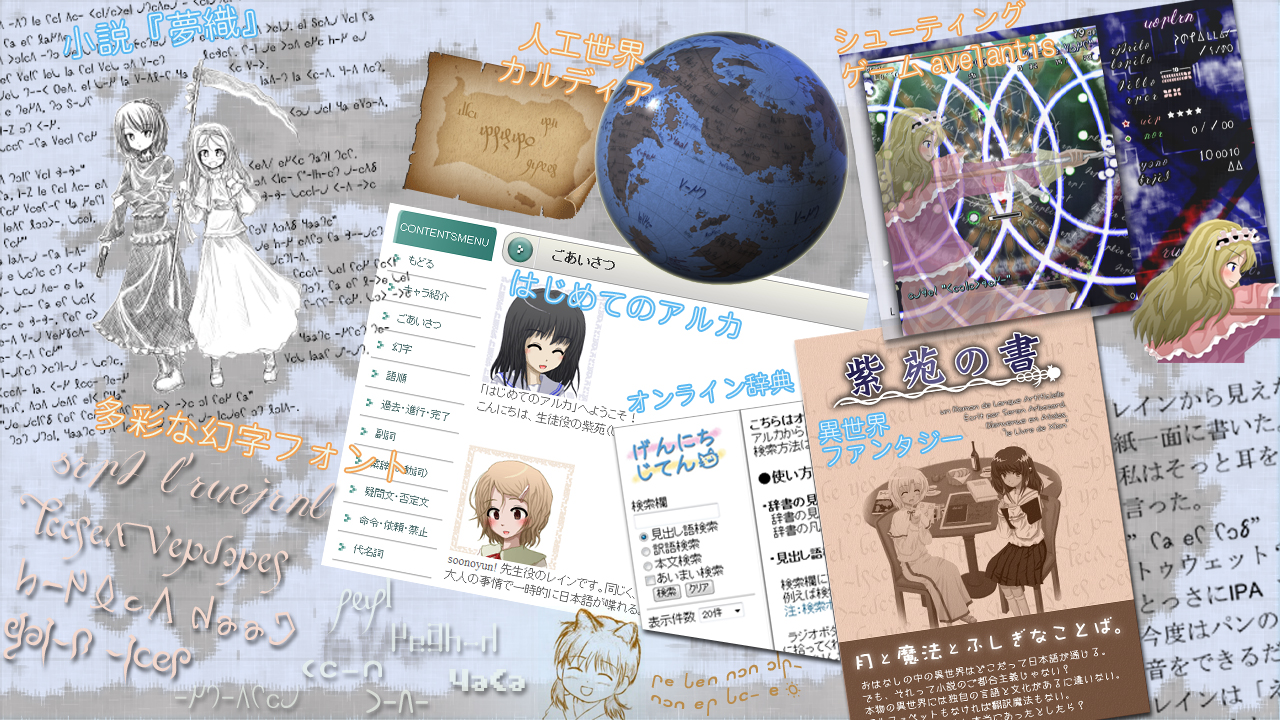
\includegraphics[width=1\textwidth]{ARKA/leis.jpg}
\end{figure}
有余裕的话,还可以看看\href{http://www44.atwiki.jp/conlang_arka/pages/1.html}{ARKA的特性}和
\textattachfile{attachfiles/語法論-人工言語の見えない心臓.pdf}{语法论-人造语言无形的心脏(日语)}
,我们也推荐\href{http://conlinguistics.org/arka/e_study_kit.html}{给初心者的指南}.

\small{
译者的话:

我翻译了初学者课程的第一部分,就是之后章节Lein的课程.但是整个网站的内容太多,我难以完全翻译.
希望有心人可以接续我的愿望.这本书以latex制成,等到网好的时候我会把所有的文档放在
\href{https://github.com/HOMODELUNA/arka-book-cn}{github}(如果访问有问题就用\href{https://gitee.com/HOMODELUNA/arka-book-cn}{gitee})上.
大家都可以来参与翻译.

\quad --亿年-二孤旋
}
\section{相关网页}

%arka维基:\url{https://arka.fandom.com/wiki/ARKA_Wiki}

Arka词典(Arka<->日语):\url{http://mindsc.ape.jp/klel/}
